% !TEX root = diss.tex

\chapter{The Relationship Between Arrhenius Pre-factors with Non-Covalent Binding}
\label{ch:arrhenius}

\section{Introduction}


DiLabio and Ingold\cite{DiLabio2005} previously investigated the formal HAT reaction of the iminoxyl/oxime self-exchange reaction. In this paper, they compiled a table of parameters from the phenomenological Arrhenius equation for a series of interesting reactions, which appear here in~\ref{tab:Arrhenius-expt}.\cite{Kreilick1966, Mader2004, Mahoney1970, DaRooge1967, Howard1973, Foti1994, Chenier1974, Chenier1975} These are thermoneutral self-exchange reactions of oxygen-centred $\pi$-radicals,\footnotemark~and other nearly thermoneutral reactions involving the destruction and formation of oxygen-centred $\pi$-radicals, reactions 3.1 and 3.2, respectively:

\begin{align}
  \ch{$\pi$-RO^. + ROH &-> ROH + $\pi$-RO^.} \hspace{2cm} \Delta H = 0 \\
  \ch{$\pi$-R}^\prime\ch{O^. + ROH &-> R}^\prime\ch{OH + $\pi$-RO^.} \hspace{2cm} \Delta H \approx 0
\end{align}

\newcommand{\tabFig}[2][0.35]{\includegraphics[scale=#1]{figures/#2.eps}}

\begin{table}[h!]
  \footnotesize
  \centering
  \caption[Table of results for (nearly) thermoneutral reactions studied.]{Table of results for (nearly) thermoneutral reactions studied. Unit for $\Delta H$, $E_a$, and calculated binding energy (BE) are \kcalmol, and $\log A$ and $k$ are \Ms.\ Adapted with permission from Reference \protect\citenum{DiLabio2005}. Copyright (2005) American Chemical Society.}
\begin{tabular}{l >{\centering}m{1.5cm} >{\centering}m{1.5cm} >{\centering}m{1.2cm} >{\centering}m{1.2cm} >{\centering}m{1.2cm} >{\centering}m{1.2cm} >{\centering}m{0.8cm} m{0em}}
  ID & \ch{RO^.}/\ch{R}$^\prime$\ch{O^.} & \ch{ROH} & $\Delta H$ & $\log~A$ & $E_a$ & $k$ & BE & \\
  \toprule
  1\cite{Kreilick1966} & \tabFig{3tBuPhO} & \tabFig{3tBuPhOH} & 0.0 & 3.7 & 1.2 & 3.3\E{2} & -10.8 &\\
  2\cite{Mader2004} & \tabFig{4MeC5H4ONO} & \tabFig{4MeC5H6NOH} & -2.0 & 3.8 & 3.8 & 10 & -14.8 &\\
  3\cite{Kreilick1966} & \tabFig[0.4]{2tBuNO} & \tabFig[0.4]{2tBuNOH} & 0.0 & 5.1 & 3.5 & 3.3\E{2} & -10.1 &\\
  4\cite{Mahoney1970,DaRooge1967} & \tabFig{3tBuPhO} & \tabFig{tBuPhOH} & 4.2 & 5.5 & 4.8 & 93 & -10.0 &\\
  5\cite{Howard1973} & \tabFig[0.7]{tBuOO} & \tabFig{3tBuPhOH} & -7.0 & 4.2 & 0.5 & 7\E{3} & -6.8 &\\
  6\cite{Kreilick1966} & \tabFig[0.7]{Ph2NO} & \tabFig[0.7]{Ph2NOH} & 0.0 & $>$7 & - & $>$10$^7$ & -14.8 &\\
  7\cite{Foti1994} & \tabFig{PhO} & \tabFig{2hydroxynaphthalene} & -2.2 & 8.3 & 2.3 & 4\E{6} & -8.6 &\\
  8\cite{Chenier1974} & \tabFig[0.7]{tBuOO} & \tabFig{PhOH} & 0.3 & 7.2 & 5.2 & 3\E{3} & -5.5 &\\
  9\cite{Chenier1974} & \tabFig[0.7]{tBuOO} & \tabFig{2hydroxynaphthalene} & -1.9 & 6.4 & 2.6 & 3\E{4} & -5.6 &\\
  10\cite{Chenier1975} & \tabFig[0.7]{tBuOO} & \tabFig{alphatetralinperoxide} & 1.4 & 6.0 & 4.5 & 7\E{2} & -8.0 &
\end{tabular}
\label{tab:Arrhenius-expt}
\end{table}

\footnotetext{\noindent A $\pi$-radical is one in which the SOMO is orthogonal to the plane of the molecular framework, i.e.\ of $\pi$-symmetry. Note that free alkoxyl radicals cannot be distinguished as either $\sigma$ or $\pi$-radicals, as the SOMO is degenerate, or free to rotate with respect to the rest of the molecular framework. Therefore, only the geometry of the radical-molecule complex can resolve the symmetry of the SOMO.}

Although it is well known that reactions of this nature involve remarkably low activation energies ($E_a$),\cite{Lucarini1996,Mahoney1970a,Mahoney1975,Korcek1972} they also have unusually low Arrhenius pre-exponential factors ($A$), or as we shall refer to them, \emph{A-factors}. As a result, these reactions are generally slower than expected, evidence for which is summarised in~\ref{tab:Arrhenius-expt}.
The measured A-factors range from $10^{3.5}$--$10^{8.3}$ \Ms, while HAT reactions are typically $10^{8.5\pm0.5}$ \Ms.\cite{Benson1976} In this past,  this has been attributed to steric shielding around the oxygen atoms, resulting in a large entropic barrier.\cite{DiLabio2005} Additionally, it was noted that the degree of steric shielding on the oxygen atom appears to play an important role in the order of the A-factor; systems with greater bulk have lower A-factors, while non-shielded systems have larger A-factors.

Steric-electronic effects are known to play an important role in HAT, and have been studied extensively.\cite{Finn2004,Salamone2011,Pischel2001,Griller1981,Bietti2011, Salamone2012,Malatesta1982,Salamone2014} Although the abstraction of a specific bond may be more thermodynamically favourable than others on a given substrate, if it is not accessible due to steric constraints, abstraction will not occur at this site. Otherwise, additional steric bulk can lead to significant reductions in reactivity, through destabilisation of the TS complex. For example, in reactions of tertiary acetamides with \cumo,\cite{Salamone2014} where abstraction occurs mainly from C-H bonds $\alpha$ to the nitrogen atom, a two-fold decrease in the normalised rate constant is observed in going from $N,N$-dimethylacetamide to $N,N$-diisobutylacetamide ($k_H$ = $2.0 \times 10^5$ and $7.8 \times 10^4$ \Ms, respectively).

Upon first inspection, all of the reactions in~\ref{tab:Arrhenius-expt} appear to be of a similar nature. Each reaction involves the formation and destruction of O-H bonds as the thermodynamic driving force. All of these bonds expected to be of comparable strength, therefore, differences should not contribute significantly to reaction barriers in a Bell-Evans-Polanyi principle fashion. Hence, the large degree of variance in their rate constants ($k$) is somewhat surprising. For the closely related self-exchange reaction between phenol and phenoxyl,\cite{Mayer2002} a strong molecule-radical pre-reaction complex is formed, ca. 10 \kcalmol below the separated reactants. It is therefore expected that most, if not all, of the systems in~\ref{tab:Arrhenius-expt} should exhibit a similar molecule-radical complex, granted, the strength of the interaction will vary because of steric repulsion.

Currently, there is no literature which describes the relationship between the pre-reaction complex and the kinetics of a reaction. Using the reactions and data in~\ref{tab:Arrhenius-expt}, we ask the question: \emph{Do A-factors have a correlation with non-covalent binding energies of the pre-reaction complex?} This is a reasonable question as non-covalent binding and steric hinderance represent a loss of degrees of freedom and therefore entropy,\footnotemark~which ultimately determines the A-factor magnitude. If the answer to the question is yes, then non-covalent binding may be useful as a diagnostic for the ``looseness'' or ``tightness'' of a TS complex, in addition to providing an important link between theory and experiment.

\footnotetext{Recall from Equation~\ref{eq:afactor} that the A-factor can be related to TST such that the primary variable is entropy ($\Delta^\ddagger S^0$).}

\section{Computational methods and details}

Density-functional theory (DFT) calculations were carried out using the Gaussian-09 software package.\cite{Frisch2009} Care was taken to obtain minimum energy structures through detailed conformational analysis. For this, I utilised the BLYP density-functional\cite{Becke1988,Lee1988} paired with the empirical D3 dispersion correction\cite{Grimme2010} with the recommended Becke-Johnson damping functions,\cite{Johnson2006} as well as our groups' own \emph{basis set incompletion potentials} (BSIPs),$^*$\jnote{update citation} and minimal MINIs basis sets.\cite{Huzinaga1984} The use of minimal basis sets corrected for basis set incompleteness allows DFT-based methods (as opposed to semi-empirical or force-field based approaches) to be used efficiently in performing a large number of calculations. Minimum energy conformers of the monomers (substrates and radicals) were first obtained by manual manipulation of the necessary dihedral bond angles, followed by geometry optimisation and vibrational analysis.

The lowest energy radicals and substrates were combined to generate the appropriate pre-reaction complexes. These pre-reaction complexes were subject to conformational analysis using the same BLYP-D3(BJ)-BSIP/MINIs method. Geometries were initially manipulated by hand. It became apparent that manual manipulation resulted in an unsatisfactory exploration of the conformational space. To solve this, all the necessary dihedral angles were scanned systematically using a combination of scripts.\cite{note5} All manipulated geometries were subject to optimisation. For each complex, the top 5--10 complex geometries were subject to further optimisation using a higher level of theory (BLYP-D3(BJ)/pc-1) to obtain the final minimum energy pre-reaction complex structures. Due to the free rotation of $t$-butyl and methyl groups, some of the optimised pre-reaction complex structures contain small imaginary frequencies, and thus do not represent proper stationary states. Several measures were taken to resolve this, however, no resolution was obtained. Regardless, the complexes adequately represent the pre-reaction complex and differences in ``true'' binding energies should be negligible.

To obtain accurate pre-reaction complex binding energies, the substrates and complexes were subject to single-point energy calculations using the LC-$\omega$PBE long-range corrected density functional\cite{Vydrov2006,Vydrov2006a} with D3(BJ) dispersion corrections and pc-2 basis sets with truncated $f$-type functions (pc-2-spd).\cite{Johnson2013} This method was selected on the recommendation of work by \citet{Johnson2013}, which demonstrated the accuracy of this method for the calculation of NCIs. On the basis of the reported mean absolute error in Reference \citenum{Johnson2013} for the S66 benchmark set of sixty-six different non-covalently interacting dimers,\cite{Rezac2011} the calculated binding energies reported herein from the LC-$\omega$PBE-D3(BJ)/pc-2-spd level of theory carry an estimated 0.2 \kcalmol margin of error.

\section{Results and discussion}

The theoretically determined electronic binding energies calculated for the lowest energy pre-reaction complex of each system are listed in~\ref{tab:Arrhenius-expt}. The logarithm of A-factor against binding energy was plotted, as shown in~\ref{fig:Arrhenius}. The overall correlation is quite poor ($R^2$=0.33), however, the majority of the data is grouped about a single, well correlated line ($R^2$=0.95). Interestingly, the intercept of the fitted line which corresponds to zero binding energy is 8.63, a result which is in line with the observed A-factor in ``normal'' HAT reactions, \emph{viz. }$10^{8.5\pm0.5}$ \Ms.\cite{Benson1976} This suggests that the observed correlation is valid, that is, NCIs may have an impact on A-factors. I shall demonstrate that the data which do not correlate are reasonable outliers. In fact, using simple rational I shall demonstrate that different regimes of sterics result in different processes leading to the TS complex. As a result, deviations from the relationship between A-factor and binding energy are observed.

\begin{figure}[htb]
  \centering
  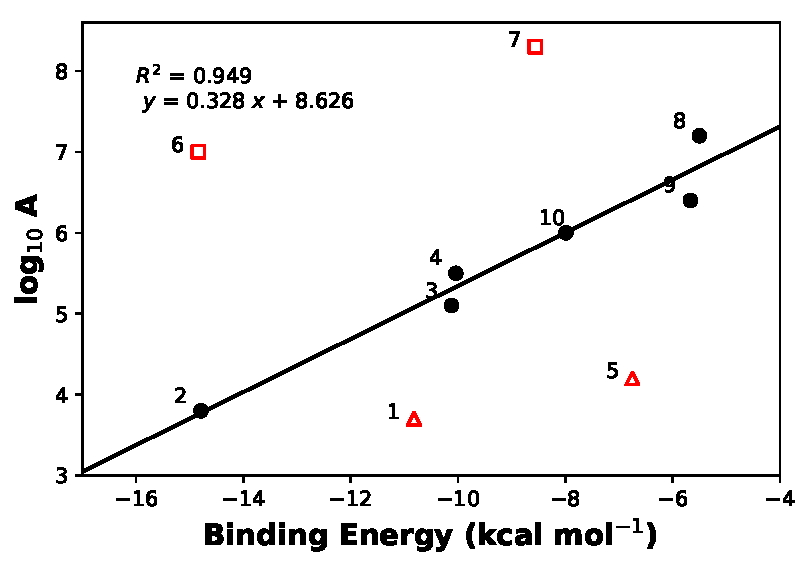
\includegraphics[width=0.85\textwidth]{figures/arrhenius-scatter.pdf}
  \caption[Plot of logarithm of A-factor against binding energy.]{Plot of logarithm of A-factor against binding energy. Black points only were included in the line fitting (slope = 0.328 \kcalmol, intercept = 8.626 \kcalmol, and $R^2$ = 0.949). Red points with open faced markers indicate outliers, \emph{vide infra}. The inclusion of complexes 1, 5, and 7 result in an $R^2$=0.334. Complex 6 is always omitted as the experimental A-factor is approximate.}
\label{fig:Arrhenius}
\end{figure}

In order to illustrate this, consider the fundamental properties of the HAT reaction involved here; the two important concerted reaction mechanisms which can occur, direct HAT and PCET.\@ Specifically, we must consider the geometric constraints in which these reactions occur. For direct HAT to occur, the SOMO of the radical must overlap with the O-H $\sigma^*$ anti-bonding orbital. Often this requires the rotation of the hydroxyl group out of the plane, the barrier to which can be as much as 3.1 \kcalmol on the basis of the rotational barrier in phenol.\cite{Kim1994} In PCET, there are two possibilities: the SOMO of the radical must be able to overlap with the corresponding oxygen $p$-orbital, as seen in the work of \citet{Mayer2002}; or a lone pair-$\pi$ or $\pi$-$\pi$ overlap must occur, as seen in the work of \citet{DiLabio2007}. Due to time constraints, I did not seek to obtain TS complex structures. Nonetheless, from the pre-reaction complex one can surmise as to the TS complex. Thus, by applying these basic principles, it is possible to rationalise the trend observed in~\ref{fig:Arrhenius}.

\begin{figure}[!h]
\centering
\hspace*{-1.8cm}
\begin{minipage}{8cm}
  \centering
  \begin{overpic}[width=\textwidth]{figures/complex2_hbond}
  \put(5,91) {\large\textbf{A.}}
\end{overpic}
\end{minipage}%
\begin{minipage}{8cm}
  \centering
  \begin{overpic}[width=\textwidth]{figures/complex3_hbond}
  \put(5,90) {\large\textbf{B.}}
\end{overpic}
\end{minipage}
\caption[Three-dimensional stuctures of pre-reaction complexes 2 (TEMPO-H and 4-oxo-TEMPO) and 3 (di-$t$-butyl-hydroxylamine and di-$t$-butyl-nitroxyl).]{Three-dimensional structures of \textbf{A} complex 2, and \textbf{B} complex 3. Hydrogen bond distances are shown in units of \AA.\@ The elements are coloured as white for carbon, light blue for hydrogen, red for oxygen, and blue for nitrogen.}
\label{fig:com2-3}
\end{figure}

We shall begin by examining the points which fall on the expected line, complexes 2--4 and 8--10, all of which require small conformational changes to proceed through HAT reactions. Complexes 2 and 3 and shown in~\ref{fig:com2-3}, and are very similar in structure, both are hydroxylamine-nitroxyl couples with similar degrees of steric bulk adjacent to the reacting centres. Both the $t$-butyl and methyl groups prevent the alignment of the NO-H-ON frameworks in a PCET manner. Additionally both pre-reaction complexes must undergo the rotation of the hydroxyl group for direct HAT.\@ In the most stable stacked conformation, complex 4 cannot undergo PCET as the steric clash of the para-position $t$-butyl groups prevent $\pi$-$\pi$ overlap. In order to react $via$ HAT, the hydroxyl group must rotate out of the plane. Alternatively, an open conformation for complex 4 is possible, which lies ca. 2 \kcalmol higher in energy than the stacked complex, a result which is also consistent with the observed trendline. From the open conformation, PCET is still not possible due to the steric bulk of the ortho-position $t$-butyl groups of the radical, thus this reaction likely proceeds through direct HAT.\@

\begin{figure}[htb]
\centering
\hspace*{-1.8cm}
\begin{minipage}{8cm}
  \centering
  \begin{overpic}[width=\textwidth]{figures/complex4_hbond}
  \put(0,100) {\large\textbf{A.}}
\end{overpic}
\end{minipage}%
\begin{minipage}{8cm}
  \centering
  \begin{overpic}[width=\textwidth]{figures/complex4_steric}
  \put(0,100) {\large\textbf{B.}}
\end{overpic}
\end{minipage}
\caption[Three-dimensional stucture of pre-reaction complex 4 between 2,4,6-tri-$t$-butylphenol and  4-$t$-butylphenoxyl.]{Three-dimensional structure of pre-reaction complex 4 between 2,4,6-tri-$t$-butylphenol and  4-$t$-butylphenoxyl. \textbf{A} demonstrates the hydrogen bond distances in units of \AA, and the out-of-plane rotation by 35.2$^\circ$ of the phenolic hydroxyl group. \textbf{B} demonstrates the steric clash (highlighed by red box) between the para-position $t$-butyl groups. The elements are coloured as white for carbon, light blue for hydrogen, and red for oxygen.}
\label{fig:com4}
\end{figure}

Complexes 8 and 9 are similar systems, in which \ch{$t$-BuOO^.} reacts with unhindered phenolic substrates. As seen by the structures in~\ref{fig:com8-9}, the bound complexes are somewhat dissimilar. The hydroxyl group of complex 8 is rotated out of the plane 24$^\circ$, while this is not true for complex 9. It is likely that the larger aromatic system of 2-naphtol results in a larger OH rotational barrier, and thus the most favourable conformation is entirely in the plane. Complex 8 was previously studied by \citet{DiLabio2007}, where it was demonstrated that a partial bonding interaction exists between the peroxyl lone-pair and phenolic $\pi$-system, giving a PCET mechanism. Although the pre-reaction complexes are somewhat dissimilar, the conformational changes necessary to reach the PCET TS complex, similar to that reported in reference \citenum{DiLabio2007}, are likely not dramatically different in terms of energetic barriers. Any small differences that are observed result in noise in the observed trend.

\begin{figure}[htb]
\centering
\hspace*{-1.8cm}
\begin{minipage}{8cm}
  \centering
  \begin{overpic}[width=\textwidth]{figures/complex8_hbond}
  \put(0,100) {\large\textbf{A.}}
\end{overpic}
\end{minipage}%
\begin{minipage}{8cm}
  \centering
  \begin{overpic}[width=\textwidth]{figures/complex9_hbond}
  \put(0,100) {\large\textbf{B.}}
\end{overpic}
\end{minipage}
\caption[Three-dimensional stuctures of pre-reaction complexes 8 ($t$-butylperoxyl and phenol) and 9 ($t$-butylperoxyl and 2-naphthol).]{Three-dimensional stuctures of pre-reaction complexes \textbf{A.} 8 ($t$-butylperoxyl and phenol) and \textbf{B.} 9 ($t$-butylperoxyl and 2-naphthol). Hydrogen bond distances are shown in units of \AA.\@ Complex 8 has an out of plane rotation of the phenolic hydroxyl group of 24.1$^\circ$/ The elements are coloured as white for carbon, light blue for hydrogen, and red for oxygen.}
\label{fig:com8-9}
\end{figure}

Complex 10 is unique in that it is the only reaction between a peroxide and a peroxyl radical. The self-exchange reaction between \ch{HOO^.} and \ch{HOOH} can be considered the simplest reference for the reaction of $\alpha$-tetralin peroxide with $t$-butylperoxyl. To the best of my knowledge, the mechanism of the hydroperoxyl-hydrogen peroxide couple has not been characterised previously in the literature, although the TS structure has been previously reported.\cite{Isborn2005} Using this structure, calculations reveal a lone pair-lone pair interaction leading to partial bonding in the TS, i.e.\ a PCET mechanism. Details of this can be found in Appendix X. For complex 10 to achieve the same lone pair-lone pair interaction, the two species must rotate by approximately 30$^\circ$ relative to one another. This is somewhat unfavourable due to steric clash.

\begin{figure}[htb]
\centering
\hspace*{-1.8cm}
\begin{minipage}{8cm}
  \centering
  \begin{overpic}[width=\textwidth]{figures/complex4_hbond}
  \put(0,100) {\large\textbf{A.}}
\end{overpic}
\end{minipage}%
\begin{minipage}{8cm}
  \centering
  \begin{overpic}[width=\textwidth]{figures/complex4_steric}
  \put(0,100) {\large\textbf{B.}}
\end{overpic}
\end{minipage}
\caption[Three-dimensional stucture of pre-reaction complex 10 between $t$-butylperoxyl and $\alpha$-tetralin peroxide.]{Three-dimensional stucture of pre-reaction complex 10 between $t$-butylperoxyl and $\alpha$-tetralin peroxide. \textbf{A} demonstrates the hydrogen bond distances in units of \AA, and the out-of-plane rotation by 35.2$^\circ$ of the phenolic hydroxyl group. \textbf{B} demonstrates the steric clash (highlighed by red box) between the para-position $t$-butyl groups. The elements are coloured as white for carbon, light blue for hydrogen, and red for oxygen.}
\label{fig:com10}
\end{figure}

\jnote{Add HOOH-OOH TS details to appendix}
\begin{figure}[htb]
  \centering
  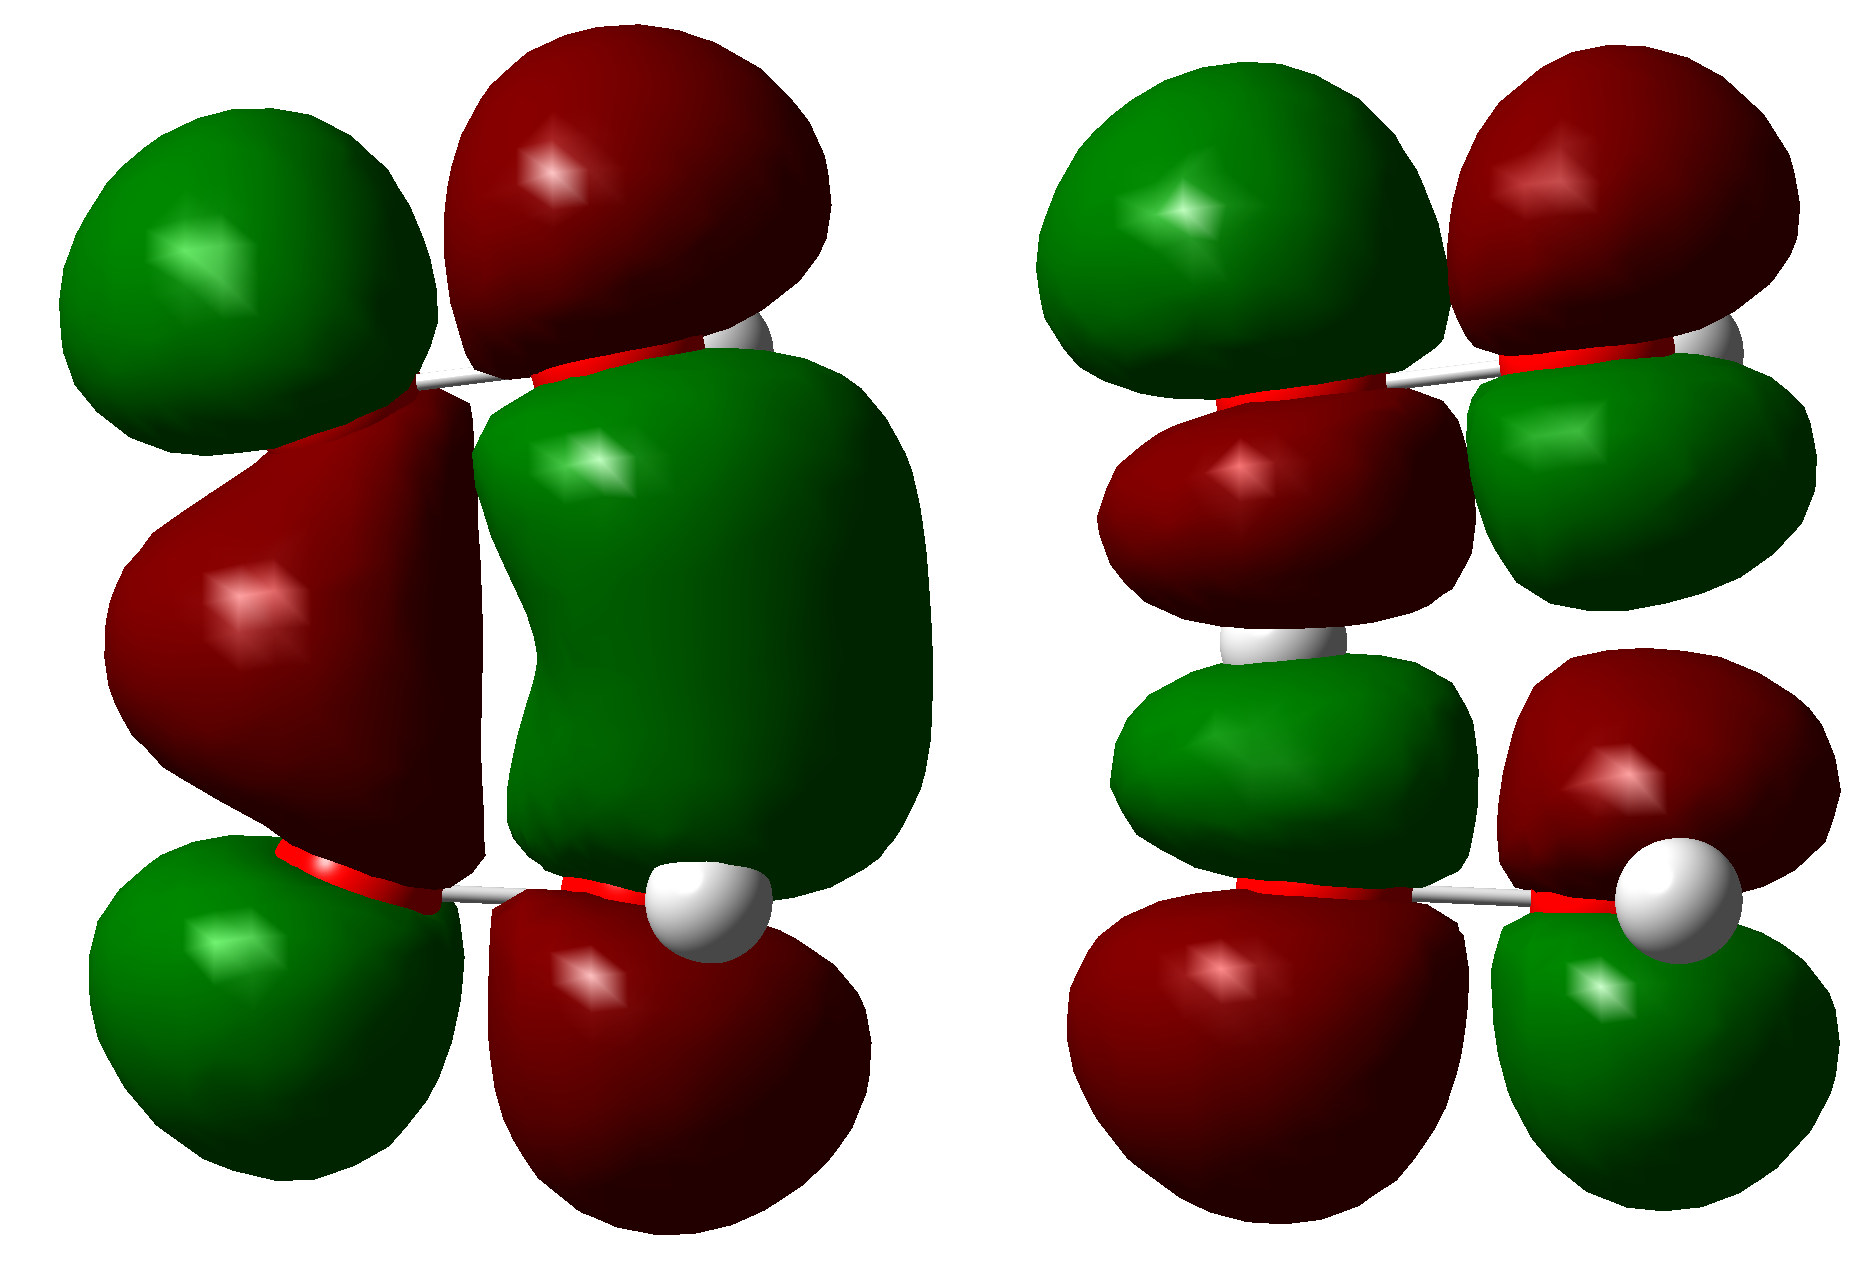
\includegraphics[width=\textwidth]{figures/hoohooh_TS.png}
  \caption[Molecular orbitals of hydrogen peroxide-peroxyl self-exchange reaction TS complex, demonstrating a PCET mechanism.]{Molecular orbitals of hydrogen peroxide-peroxyl self-exchange reaction TS complex, demonstrating a PCET mechanism. Left is the HOMO-1 and right is the SOMO.\@ Together they demonstrate a lone pair-lone pair net half bonding interactions, consitent with PCET.}
\end{figure}

All the the complexes which follow the observed trend must undergo an additional process with a barrier that is likely about 3 \kcalmol (on the basis of the phenolic rotational barrier) to reach the TS complex. This is illustrated in in~\ref{fig:afactor-trend}.

\begin{figure}[htb]
  \centering
  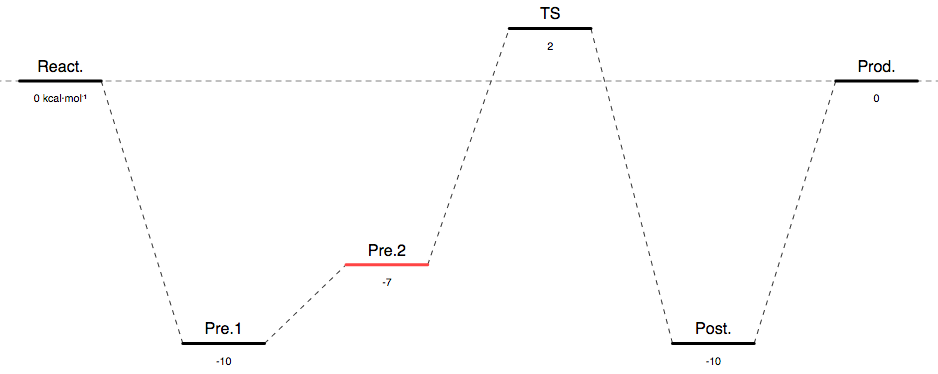
\includegraphics[width=\textwidth]{figures/afactor-trend.png}
  \caption[Reaction coordinate illustrating a conformational change to a second pre-reaction complex prior to transition state.]{Reaction coordinate illustrating a conformational change to a second pre-reaction complex prior to transition state. All energies are arbitrarily estimated based on the phenol-phenoxyl self-exchange reaction. React. = reactants, Pre.1 = lowest energy pre-reaction complex, Pre.2 = postulated higher energy pre-reaction complex, TS = transition state, Post. = post-reaction complex, Prod. = products.}
\label{fig:afactor-trend}
\end{figure}

Consider next the points which sit above the trendline, complexes 6 and 7. The A-factor for complex 6 is approximate and thus does not get factored into the line fitting. In both cases, the non-covalently bound complexes are in a slipped-parallel $\pi$-stacked conformation. Complex 7 in particular is very similar to the phenol-phenoxyl couple, except with 2-naphthol instead of phenol. Therefore, it is possible to infer that both of these reactions take place through a PCET mechanism. Specifically, these pre-reaction complexes do not require an additional conformational change to approach the TS complexes, as illustrated in~\ref{fig:afactor-direct}.

\begin{figure}[htb]
  \centering
  
\includegraphics[width=\textwidth]{figures/afactor-direct.png}
  \caption[Reaction coordinate illustrating no conformational change before moving to the transition state.]{Reaction coordinate illustrating no conformational change before moving to the transition state. All energies are arbitrarily estimated based on the phenol-phenoxyl self-exchange reaction. React. = reactants, Pre. = lowest energy pre-reaction complex, TS = transition state, Post. = post-reaction complex, Prod. = products.}
\label{fig:afactor-direct}
\end{figure}

Finally, consider the points which fall below the trendline, complexes 1 and 5. In both cases, a high degree of steric repulsion likely does not allow for a PCET mechanism. Complex 1 is the reaction with the most steric shielding surrounding the reaction centres, with four ortho-position $t$-butyl groups in total. As a result, the most stable pre-reaction complex does not have a hydrogen bond, which is unique among the ten reaction couples studied here. A higher energy (0.6 \kcalmol) pre-reaction complex 1 does exist, and possesses an open conformation hydrogen bond. This higher energy conformer is likely that which leads to HAT through a direct mechanism. The geometry is such that the hydrogen group must rotate and the $t$-butyl groups must approach one another to approach the TS complex. This higher energy complex is still inconsistent with the trendline.

Complex 5 possesses an unusual hydrogen bond. Normally hydrogen bonds are nearly linear so that there is both a dipole-dipole interaction and an orbital interaction such that the lone pair of the acceptor donates electron density into the OH $\sigma^*$ anti-bonding orbital.\cite{Jeffrey1997} In the case of complex 5, the hydrogen bond is nearly perpendicular, resulting in only an orbital interaction.\footnotemark~This is due to the steric repulsion between the $t$-butyl groups of $t$-butylperoxyl and 2,4,6-tri-$t$-butylphenol. This structure is comparable to of complex 8, the TS of which as published in reference \citenum{DiLabio2007}. Complex 8 which takes place through PCET, however, due to steric shielding it is apparent that complex 5 cannot conform to the correct geometry for PCET to occur. In order for this reaction to proceed, an open conformation complex must form so that a direct HAT mechanism can take place.

\footnotetext{The hydrogen bonding nature of this interaction has been verified using the NCIplot software.\cite{Johnson2010,ContrerasGarcia2011} These results can be found in Appendix X.}

For complexes 1 and 5 which fall below the trendline, the lowest energy pre-reaction complex does not correspond to one which will lead to HAT.\@ Therefore, one can describe an additional higher energy pre-reaction complex which leads to HAT, similar to the trend observed, but likely much higher in energy, as illustrated in~\ref{fig:afactor-low}.

\begin{figure}[htb]
  \centering
  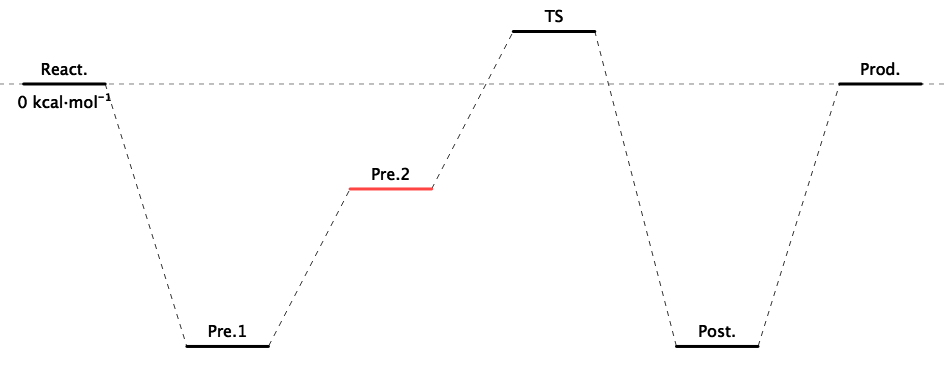
\includegraphics[width=\textwidth]{figures/afactor-low.png}
  \caption[Reaction coordinate illustrating a conformational change to a second high energy pre-reaction complex prior to transition state.]{Reaction coordinate illustrating a conformational change to a second high energy pre-reaction complex prior to transition state. All energies are arbitrarily estimated based on the phenol-phenoxyl self-exchange reaction. React. = reactants, Pre.1 = lowest energy pre-reaction complex, Pre.2 = postulated higher energy pre-reaction complex, TS = transition state, Post. = post-reaction complex, Prod. = products.}
\label{fig:afactor-low}
\end{figure}

\section{Summary}

In this investigation, I report the lowest energy pre-reaction complexes for a series of thermoneutral or nearly thermoneutral HAT reactions. I have plotted the theoretically determined electronic binding energies against the logarithm of experimentally determined A-factors. These results demonstrate that the A-factor is correlated to some extent with the binding energy, given that the reactions proceed through energetically similar pathways. The results herein can be sorted into three bins: 1. Complexes which require small conformational changes to approach the TS structure. This appears to be the most likely case for formal HAT reactions. 2. Complexes which are optimally aligned to approach the TS structure. 3. Complexes which require a large conformational change to approach the TS structure.

These results suggest that different regimes of steric interactions lead to different chemical processes in seemingly similar reactions. As a results, non-covalent binding can be used as a metric for kinetics parameters, however, they cannot tell the whole story. One must first determine the relationship between the pre-reaction and TS complexes.

Additional work is necessary to extend these results. In particular, a larger sample of data points should be used. Regardless, the results herein represent a novel attempt to link theory and experiment. Given that obtaining the full PES for large molecules is computationally impractical, these results serve as a seed for developing a fundamental understanding of complex formal HAT reactions.

\newpage
\noindent \textbf{Appendix NCI Plot}
\begin{figure}[htb]
  \centering
  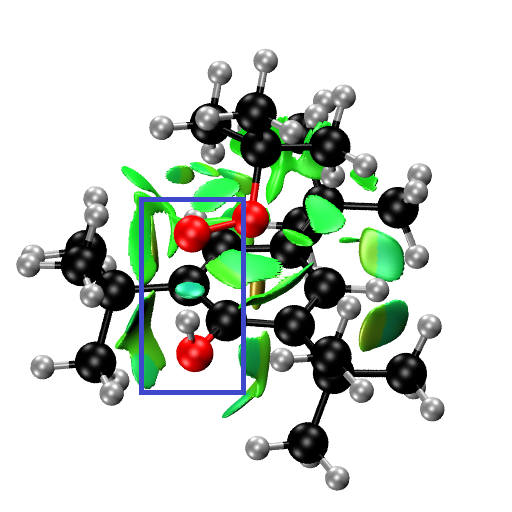
\includegraphics[width=\textwidth]{figures/nciplot.png}
  \caption{NCIplot\cite{Johnson2010,ContrerasGarcia2011} of complex 5. The blue spheroid between the $t$-butylperoxyl oxygen centred radical and the 2,4,6-tri-$t$-butylphenol hydroxyl represents hydrogen bonding.}
\end{figure}
